%% 该模板修改自《计算机学报》latex 模板
%% 主要是将双栏改成单栏,去掉了部分计算机学报标识;
%% 源文件自:https://www.overleaf.com/latex/templates/latextemplet-cjc-xelatex/ybmmymncrrmw
%% 
%%
%% This is file `CjC_template_tex.tex',
%% is modified by Zhi Wang (zhiwang@ieee.org) based on the template 
%% provided by Chinese Journal of Computers (http://cjc.ict.ac.cn/).
%%
%% This version is capable with Overleaf (XeLaTeX).
%%
%% Update date: 2023/03/10
%% -------------------------------------------------------------------
%% Copyright (C) 2016--2023 
%% -------------------------------------------------------------------
%% This file may be distributed and/or modified under the
%% conditions of the LaTeX Project Public License, either version 1.3c
%% of this license or (at your option) any later version.
%% The latest version of this license is in
%%    https://www.latex-project.org/lppl.txt
%% and version 1.3c or later is part of all distributions of LaTeX
%% version 2008 or later.
%% -------------------------------------------------------------------

\documentclass[10.5pt,compsoc,UTF8]{CjC}
\usepackage{CTEX}
\usepackage[ruled,longend,linesnumbered]{algorithm2e}
\usepackage{graphicx}
\usepackage{footmisc}
\usepackage{subfigure}
\usepackage{url}
\usepackage{multirow}
\usepackage{multicol}
\usepackage[noadjust]{cite}
\usepackage{amsmath,amsthm}
\usepackage{amssymb,amsfonts}
\usepackage{booktabs}
\usepackage{color}
\usepackage{ccaption}
\usepackage{booktabs}
\usepackage{float}
\usepackage{fancyhdr}
\usepackage{caption}
\usepackage{xcolor,stfloats}
\usepackage{comment}
\setcounter{page}{1}
\graphicspath{{figures/}}
\usepackage{cuted}%flushend,
\usepackage{captionhack}
\usepackage{epstopdf}
\usepackage{gbt7714}

%===============================%

\headevenname{\mbox{\quad} \hfill  \mbox{\zihao{-5}{ \hfill 《机器学习》  } \hspace {50mm} \mbox{2024 年 5 月}}}%
\headoddname{闵昕 \hfill 机器学习}%

%footnote use of *
\renewcommand{\thefootnote}{\fnsymbol{footnote}}
\setcounter{footnote}{0}
\renewcommand\footnotelayout{\zihao{5-}}

\newtheoremstyle{mystyle}{0pt}{0pt}{\normalfont}{1em}{\bf}{}{1em}{}
\theoremstyle{mystyle}
\renewcommand\figurename{figure~}
\renewcommand{\thesubfigure}{(\alph{subfigure})}
\newcommand{\upcite}[1]{\textsuperscript{\cite{#1}}}
\renewcommand{\labelenumi}{(\arabic{enumi})}
\newcommand{\tabincell}[2]{\begin{tabular}{@{}#1@{}}#2\end{tabular}}
\newcommand{\abc}{\color{white}\vrule width 2pt}
\renewcommand{\bibsection}{}
\makeatletter
\renewcommand{\@biblabel}[1]{[#1]\hfill}
\makeatother
\setlength\parindent{2em}
%\renewcommand{\hth}{\begin{CJK*}{UTF8}{gbsn}}
%\renewcommand{\htss}{\begin{CJK*}{UTF8}{gbsn}}





\begin{document}

\hyphenpenalty=50000
\makeatletter
\newcommand\mysmall{\@setfontsize\mysmall{7}{9.5}}
\newenvironment{tablehere}
  {\def\@captype{table}}

\let\temp\footnote
\renewcommand \footnote[1]{\temp{\zihao{-5}#1}}


\thispagestyle{plain}%
\thispagestyle{empty}%
\pagestyle{CjCheadings}

% \begin{table*}[!t]
\vspace {-13mm}


\onecolumn
\zihao{5-}\noindent 闵昕\hfill 《机器学习》\hfill 2024 年 5 月\\
\noindent\rule[0.25\baselineskip]{\textwidth}{1pt}

% \onecolumn
% \zihao{5-}\noindent 第??卷\quad 第?期 \hfill 计\quad 算\quad 机\quad 学\quad 报\hfill Vol. ??  No. ?\\
% \zihao{5-}
% 20??年?月 \hfill CHINESE JOURNAL OF COMPUTERS \hfill ???. 20??\\ 
% \noindent\rule[0.25\baselineskip]{\textwidth}{1pt}

{
\centering
\vspace {11mm}
{\zihao{2} \heiti CNN图像分类 }

\vskip 5mm

{\zihao{4}\fangsong 闵昕\quad\quad 23011210821$^{1)}$\fangsong \quad 王冠维\quad\quad 23031212262$^{2)}$}


\vspace {5mm}
\zihao{5}{$^{1)}$(西安电子科技大学杭州研究院,\quad通信工程专业,\quad卫星互联网研究所)}

\zihao{5}{$^{2)}$(西安电子科技大学杭州研究院,\quad软件工程专业,\quad先进视觉研究所)}

}



\vskip 5mm

\zihao{5}{
\setlength{\baselineskip}{16pt}\selectfont{
\noindent {\heiti 摘\quad 要\quad }
本文全面介绍了卷积神经网络(CNN)及其在FashionMNIST数据集图像分类任务中的应用。
研究首先介绍了CNN的结构和功能,强调了它们在图像处理任务中相对于全连接网络的优势。
然后,文章详细描述了一个实验,比较了不同CNN架构和学习率对模型性能的影响(2种架构*2中学习率以及一种特殊情况的学习率分析)。
结果表明,对于简单的数据集,更简单的网络结构可以有效,学习率是模型收敛和准确性的关键因素,并且根据学习率进行了优化。
文章最后提出了未来改进的建议,如预处理步骤以更好地区分特征,以及数据增强以提高模型的鲁棒性。
\par}}
\vspace {5mm}

\zihao{5}{\noindent
{\heiti 关键词 \quad }{卷积神经网络 (CNN);图像分类;网络架构;学习率;FashionMNIST 数据集 }
}
% \zihao{5-}{\heiti 中图法分类号\quad } TP\rm{\quad \quad \quad     }
% {\heiti DOI号:\quad } *投稿时不提供DOI号


\vskip 20mm


\begin{center}

\zihao{3}{ \heiti CNN Image classification}

\vspace {5mm}
\zihao{5}{  Xin Min$^{1)}$ GUANWEI WANG$^{2)}$}\\
\vspace {2mm}
\zihao{5-}{{$^{1)}$(Hangzhou Research Institute of Xidian University,\quad Major in Communication Engineering,\quad Satellite Internet Institute)}}

\zihao{5-}{{$^{2)}$(Hangzhou Research Institute of Xidian University,\quad Major in Software Engineering,\quad Advanced Visual Research Institute)}}


\end{center}

\zihao{5}{
\setlength{\baselineskip}{18pt}\selectfont{
{\bf Abstract}\quad 
\zihao{5}{\noindent This paper provides a comprehensive overview of Convolutional Neural Networks (CNNs) 
and their application in image classification tasks using the FashionMNIST dataset. 
The study begins with an introduction to the structure and function of CNNs, 
highlighting their advantages over fully connected networks in image processing tasks.
The paper then details an experiment where different CNN architectures and learning rates are compared to determine their impact on model performance. 
The results indicate that simpler network structures can be effective for straightforward datasets, 
and that learning rate is a critical factor in model convergence and accuracy.
 The paper concludes with suggestions for future improvements, 
such as preprocessing steps for better feature distinction and data augmentation for increased model robustness.
\par}}
\vspace {5mm}

{{\bf Keywords}\quad
Convolutional Neural Networks ; Image ClassificationNetwork Architecture ; Learning Rate ; FashionMNIST Dataset\par}}



%%%%%%%%%%%%%%%%%%%%%%%%%%%%%%%%%%%%%%
\zihao{5}
\vskip 50mm
% \begin{multicols}{1}


%%%%%%%%%%%%%%%%%%%%%%%%%%%%%%%%%%%%%%%%%%
%%%%%%%%%%%%%%%%%%%%%%%%%%%%%%%%%%%%%%%%%%


\section{\heiti CNN卷积神经网络}
\subsection{卷积神经网络介绍}
卷积神经网络(Convolutional Neural Networks,简称CNN)是一种具有局部连接、
权值共享等特点的深层前馈神经网络(Feedforward Neural Networks),是深度学习(deep learning)的代表算法之一,擅长处理图像特别是图像识别等相关机器学习问题
,比如图像分类、目标检测、图像分割等各种视觉任务中都有显著的提升效果,是目前应用最广泛的模型之一。

当使用全连接神经网络处理大尺寸图像时,有三个非常明显的缺点:
(1)将图像展开为向量会丢失空间信息;
(2)参数过多效率低下,训练困难;
(3)大量的参数也很快会导致网络过拟合。
卷积神经网络则可以很好地解决以上三个问题。

与常规神经网络不同,卷积神经网络的各层中的神经元是3维排列的:宽度、高度和深度。
对于输入层来说,宽度和高度指的是输入图像的宽度和高度,深度代表输入图像的通道数,
例如,对于RGB图像有R、G、B三个通道,深度为3;而对于灰度图像只有一个通道,深度为1。
对于中间层来说,宽度和高度指的是特征图(feature map)的宽和高,通常由卷积运算和池化操作的相关参数决定;
深度指的是特征图的通道数,通常由卷积核的个数决定。
全连接神经网络中的主要运算为矩阵相乘,
而卷积神经网络中主要为卷积计算。


卷积神经网络具有表征学习(representation learning)能力,
能够按其阶层结构对输入信息进行平移不变分类(shift-invariant classification),
可以进行监督学习和非监督学习,其隐含层内的卷积核参数共享和层间连接的稀疏性使得卷积神经网络能够以较小的计算量对格点化(grid-like topology)特征,
例如像素和音频进行学习、有稳定的效果且对数据没有额外的特征工程(feature engineering)要求,并被大量应用于计算机视觉、自然语言处理等领域。

如图1所示,为卷积神经网络的一个示意图:
\begin{figure}[htbp]
\centering
\centerline{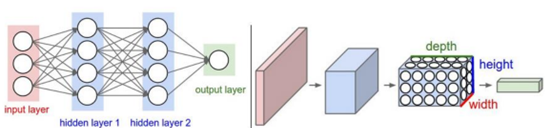
\includegraphics[width=1\linewidth]{CNN1.png}}

\heiti 图1.1\quad  卷积神经网络示例(左图为全连接层,右图为卷积层)
\label{fig1}
\end{figure}



%%%%%%%%%%%%%%%%%%%%%%%%%%%%%%%%%%%%%%%%%%
%%%%%%%%%%%%%%%%%%%%%%%%%%%%%%%%%%%%%%%%%%

\subsection{网络结构}

卷积神经网络的基本结构由以下几个部分组成:输入层(input layer),
卷积层(convolution layer),池化层(pooling layer),
激活函数层和全连接层(full-connection layer)。
具体结构如下图2所示。

\subsubsection{输入层}

在处理图像的CNN中,输入层一般代表了一张图片的像素矩阵。
可以用三维矩阵代表一张图片。三维矩阵的长和宽代表了图像的大小,
而三维矩阵的深度代表了图像的色彩通道。比如黑白图片的深度为1,
而在RGB色彩模式下,图像的深度为3。

%%%%%%%%%%%%%%%%%%%%%%%%%%%%%%%%%%%%%%%%%%
%%%%%%%%%%%%%%%%%%%%%%%%%%%%%%%%%%%%%%%%%%

\subsubsection{卷积层}

卷积神经网络的核心是卷积层,卷积层的核心部分是卷积操作。
对图像和滤波矩阵做内积(逐个元素相乘再求和)的操作就是所谓的卷积操作,
也是卷积神经网络的名字来源。卷积运算的目的是提取输入的不同特征,
第一层卷积层可能只能提取一些低级的特征如边缘、线条和角等层级,
更多层的网路能从低级特征中迭代提取更复杂的特征。

\begin{figure}[htbp]
\centering
\centerline{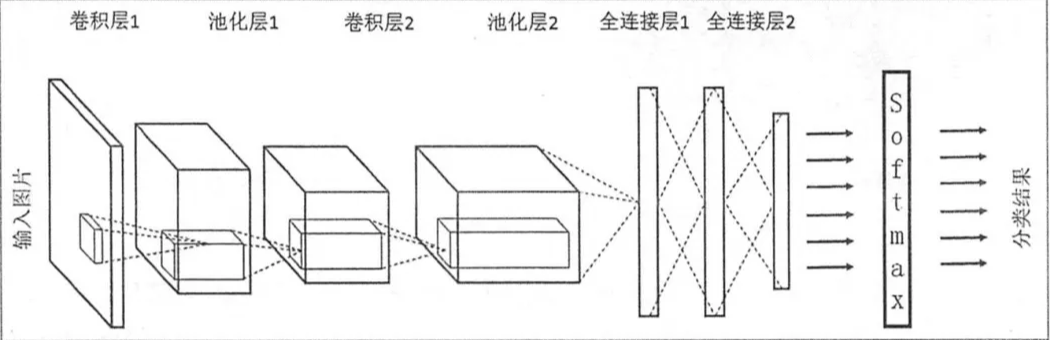
\includegraphics[width=1\linewidth]{CNN2.png}}

\heiti 图1.2\quad  卷积神经网络
\label{fig1}
\end{figure}

卷积过程实质上就是两个矩阵做乘法,在卷积过程后,原始输入矩阵会有一定程度的缩小,
比如自定义卷积核大小为3*3,步长为1时,矩阵长宽会缩小2,
所以在一些应用场合下,为了保持输入矩阵的大小,我们在卷积操作前需要对数据进行扩充,
常见的扩充方法为0填充方式,图3展示了卷积操作的基本过程。

\begin{figure}[htbp]
\centering
\centerline{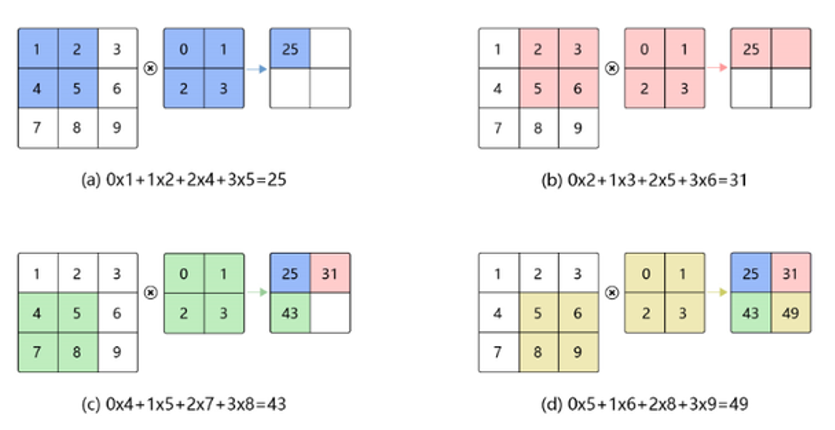
\includegraphics[width=1\linewidth]{CNN3.png}}

\heiti 图1.3\quad  卷积操作
\label{fig1}
\end{figure}

卷积层中还有两个重要的参数,分别是偏置和激活
(独立层,但一般将激活层和卷积层放在一块)。

偏置向量的作用是对卷积后的数据进行简单线性的加法,就是卷积后的数据加上偏置向量中的数据,
然后为了增加网络的一个非线性能力,需要对数据进行激活操作,在神经元中,就是将没有的数据率除掉,
而有用的数据则可以输入神经元,让人做出反应。

激活函数,最常用的激活函数目前有Relu、tanh、sigmoid,着重介绍一下Relu函数
(即线性整流层(Rectified Linear Units layer, 简称ReLU layer)),
Relu函数是一个线性函数,它对负数取0,正数则为y=x(即输入等于输出),
即f(x)=max(0,x),它的特点是收敛快,求梯度简单,但较脆弱。

\begin{figure}[htbp]
\centering
\centerline{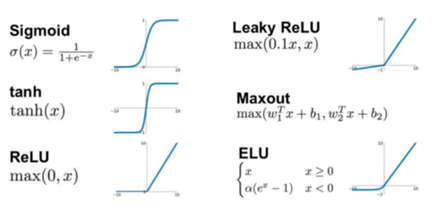
\includegraphics[width=0.6\linewidth]{CNN4.png}}
\heiti 图1.4\quad  常见的激活函数
\label{fig1}
\end{figure}

由于经过Relu函数激活后的数据0值一下都变成0,
而这部分数据难免有一些我们需要的数据被强制取消,
所以为了尽可能的降低损失,我们就在激活层的前面,
卷积层的后面加上一个偏置向量,对数据进行一次简单的线性加法,
使得数据的值产生一个横向的偏移(也就是上述所说的偏置向量),
避免被激活函数过滤掉更多的信息。

%%%%%%%%%%%%%%%%%%%%%%%%%%%%%%%%%%%%%%%%%%
%%%%%%%%%%%%%%%%%%%%%%%%%%%%%%%%%%%%%%%%%%

\subsubsection{池化层}
池化层的作用是去除冗余信息、对特征进行压缩、简化网络复杂度、减小计算量。
池化操作将输入矩阵某一位置相邻区域的总体统计特征作为该位置的输出,
主要有平均池化(Average Pooling)、最大池化(Max Pooling)等。
简单来说池化就是在该区域上指定一个值来代表整个区域。
池化层的超参数:池化窗口和池化步长。池化操作也可以看做是一种卷积操作。


\begin{figure}[htbp]
\centering
\centerline{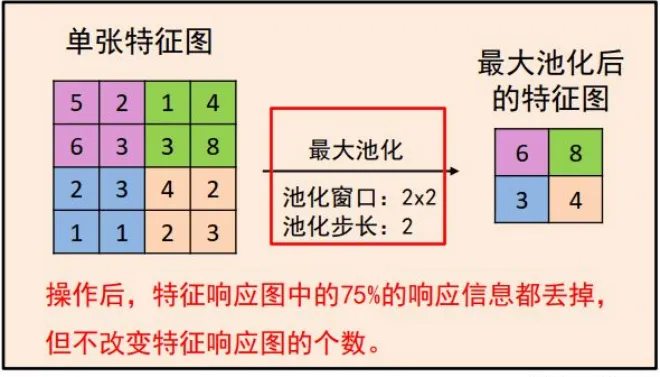
\includegraphics[width=0.6\linewidth]{CNN5.png}}
\heiti 图1.5\quad  Max Pool图解
\label{fig1}
\end{figure}
池化层夹在连续的卷积层中间, 用于压缩数据和参数的量,减小过拟合。
简而言之,如果输入是图像的话,那么池化层的最主要作用就是压缩图像。
池化层的作用是对数据进行降维处理,对于所有神经网络来说,
随着网络深度增加,网络中权值参数的数量也会越来越大,
这也是导致我们在训练一个大型网络时必须使用大型服务站和GPU加速了,
但是卷积神经网络出了它本身权值共享和局部连接方式可以有效的降低网络压力外,
池化层也作为一个减低网络压力的重要组成部分,
经过卷积层后的数据做为池化层的输入进行池化操作。

总而言之,池化层的基本作用有三种:
①特征不变性(图像处理中经常提到的特征的尺度不变性)
②特征降维(提取重要信息去除冗余信息)
③在一定程度上防止过拟合
%%%%%%%%%%%%%%%%%%%%%%%%%%%%%%%%%%%%%%%%%%
%%%%%%%%%%%%%%%%%%%%%%%%%%%%%%%%%%%%%%%%%%

\subsubsection{全连接层}

在经过多轮卷积层和池化层的处理之后,在CNN的最后一般会由1到2个全连接层来给出最后的分类结果。
经过几轮卷积层和池化层的处理之后,可以认为图像中的信息已经被抽象成了信息含量更高的特征。
我们可以将卷积层和池化层看成自动图像特征提取的过程。
在提取完成之后,仍然需要使用全连接层来完成分类任务。

\subsubsection{SoftMax层}

Softmax 层通常被用作神经网络输出层的激活函数,
特别是在多类别分类问题中。
它的作用是将原始的类别分数转化为概率分布,
使得所有类别的概率之和为 1。
这样,神经网络的输出可以被解释为每个类别的概率。

\begin{figure}[htbp]
\centering
\centerline{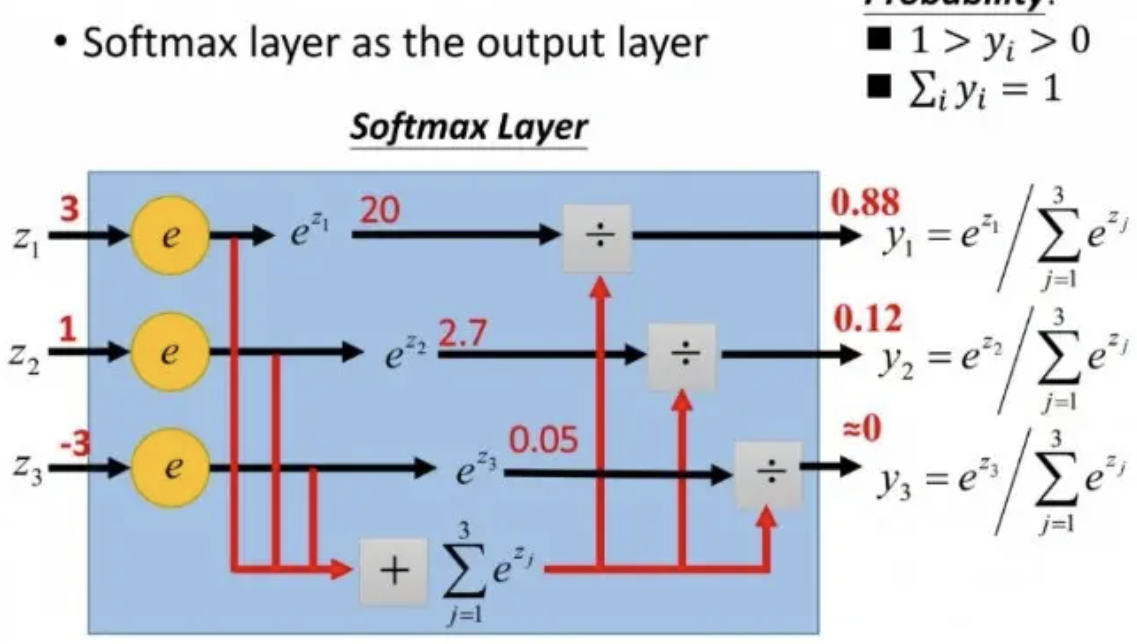
\includegraphics[width=0.6\linewidth]{CNN6.png}}
\heiti 图1.6\quad  Softmax图解
\label{fig1}
\end{figure}

值得注意的是,在Softmax层中,由于经过指数函数,
两两概率之间的距离其实是被放大的。

如何评估一个模型的好坏,
在分类问题中,最常见的定义损失函数的方式为交叉熵(Cross Entropy)。
一般交叉熵会和Softmax一起使用,这两个函数一般都定义在Softmax层

%%%%%%%%%%%%%%%%%%%%%%%%%%%%%%%%%%%%%%%%%%
%%%%%%%%%%%%%%%%%%%%%%%%%%%%%%%%%%%%%%%%%%

\subsubsection{总结}

上述我们已经叙述了在CNN网络中各个层的作用,在实际的训练过程中,
主要包括前向传播和反向传播两个过程。
在前向传播阶段,选取训练样本(x,y),将x输入网络中。随机初始化权值(一般情况下选取小数),
信息从输入层经过一层一层的特征提取和转换,最后到达输出层,
得到输出结果。
在反向传播阶段,输出结果与理想结果对比,计算全局性误差(即Loss)。
得到的误差反向传递给不同层的神经元,按照“迭代法”调整权值和偏重,
寻找全局性最优的结果。

如图7所示,便为整个训练流程。

 

\begin{figure}[htbp]
\centering
\centerline{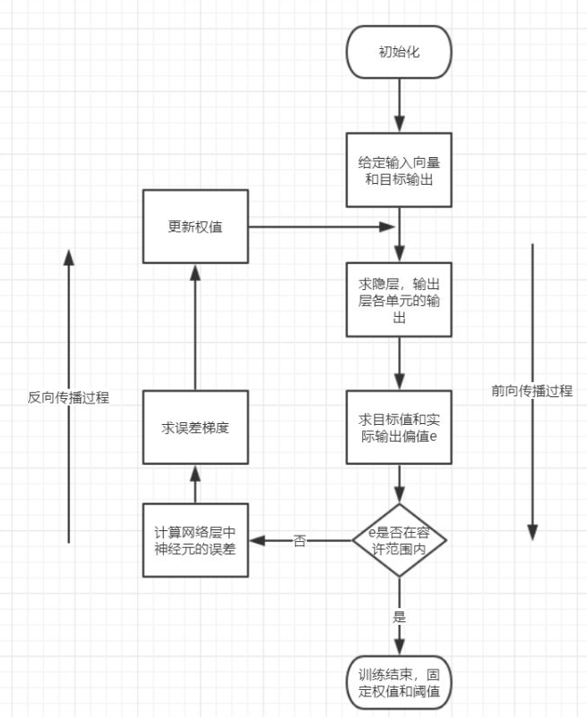
\includegraphics[width=0.5\linewidth]{CNN7.png}}
\heiti 图1.7\quad  CNN流程总结
\label{fig1}
\end{figure}

%%%%%%%%%%%%%%%%%%%%%%%%%%%%%%%%%%%%%%%%%%
%%%%%%%%%%%%%%%%%%%%%%%%%%%%%%%%%%%%%%%%%%

\section{\heiti 利用CNN实现FashionMNIST数据集的图像分类任务}

\subsection{实验要求}
(1) 数据集:FashionMNIST

(2) 基础要求:利用CNN网络实现分类任务,按照标准划分,进行训练和测试

(3) 性能指标:准确率(Acc)、收敛速度等

%%%%%%%%%%%%%%%%%%%%%%%%%%%%%%%%%%%%%%%%%%

\subsection{实验步骤}

\subsubsection{数据处理}

1.使用FashionMNIST数据集,将数据集分为80$\%$的训练集和20$\%$的测试集;

2.由于图像为灰度图,所以通道数为1;

3.将数据分为64个batch;(将数据集分为多个小数据集的优点:
①利用GPU并行处理的能力提高训练速度
②减少每次需要计算的数据量,减少内存)

4.设置25个Epoch;
(通过多个epoch的训练,模型有机会逐渐减小损失并提高性能,因为每个epoch都会进行参数的微调和优化。)

5.将测试集归一化灰度同除255。(归一化有可能提高数据精度)

%%%%%%%%%%%%%%%%%%%%%%%%%%%%%%%%%%%%%%%%%%

\subsubsection{训练模型1——构建基础卷积神经网络架构}

通过第一章的介绍,我们了解了神经网络的基本架构,包括输入层,卷积层,池化层,全连接层,SoftMax层,
在最初的考虑中我们采用如图2.1所示的网络架构:


\begin{figure}[htbp]
\centering
\centerline{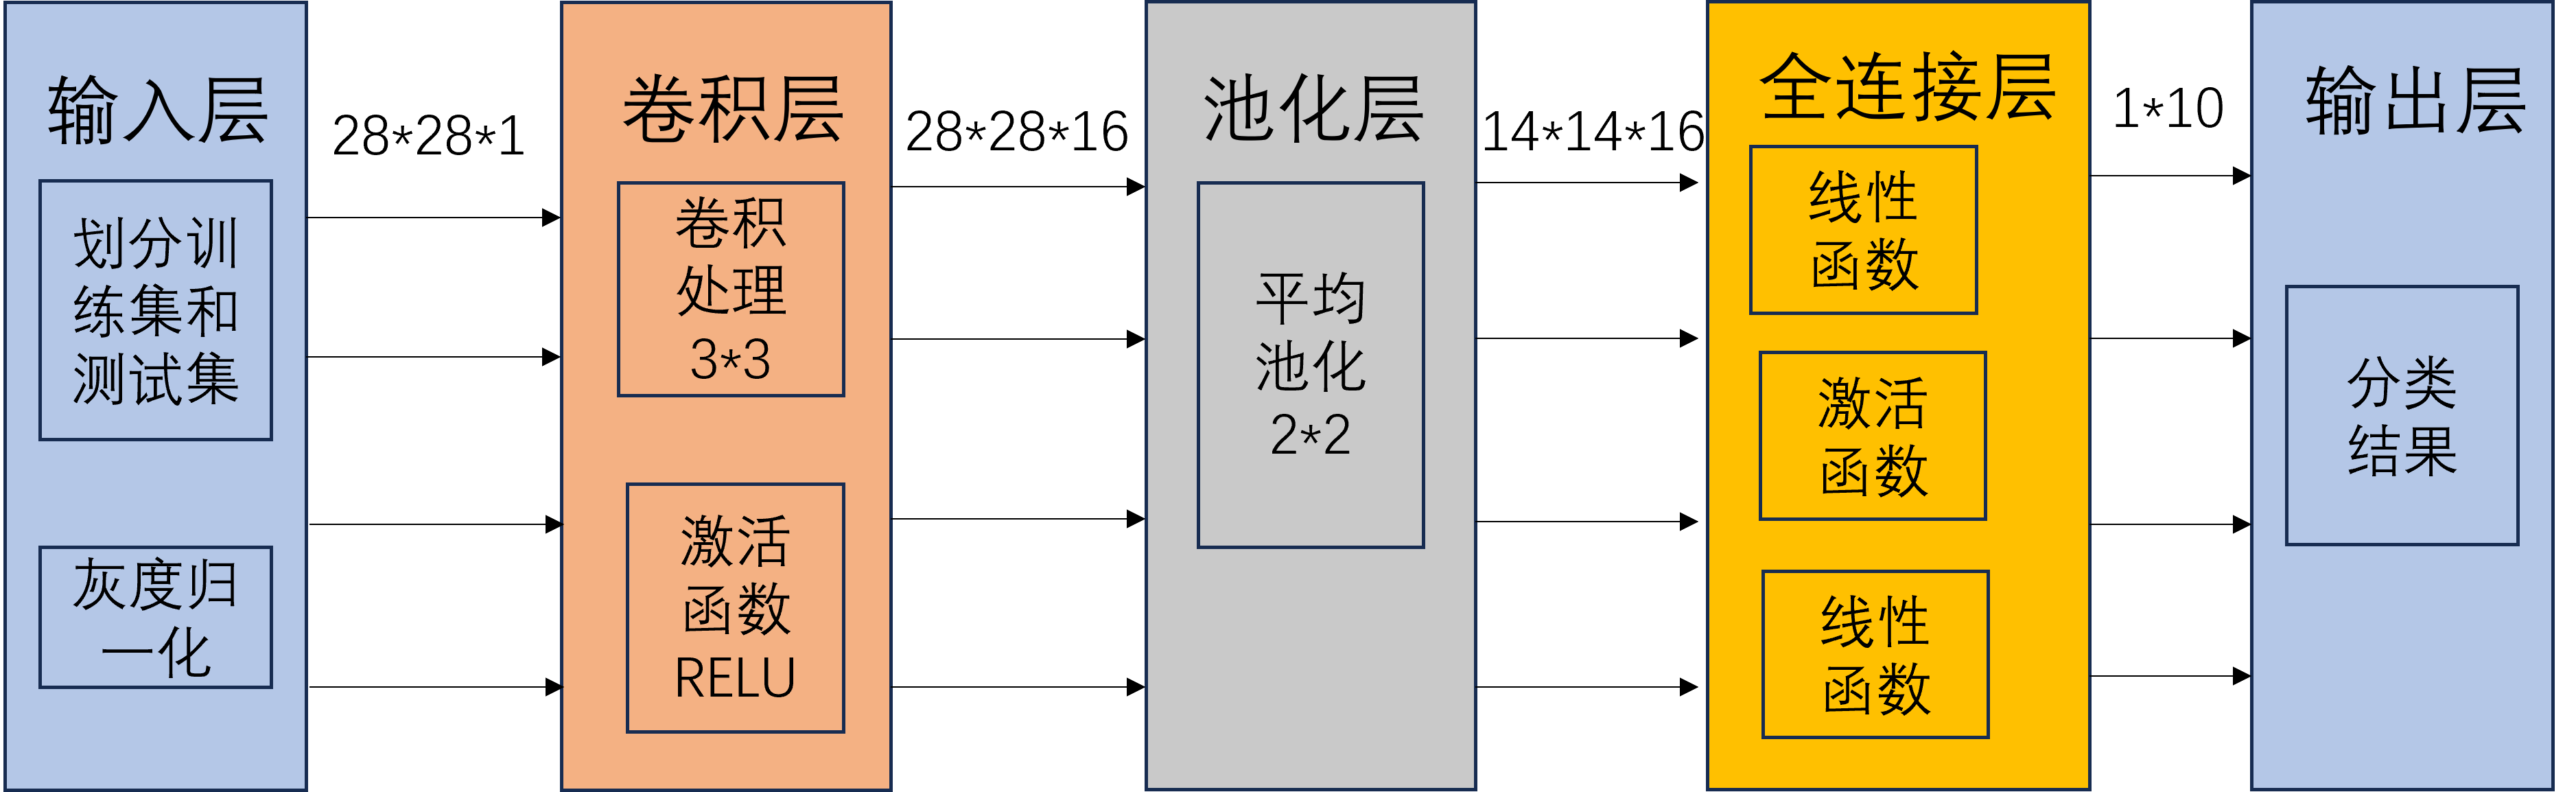
\includegraphics[width=1\linewidth]{CNN21.png}}
\heiti 图2.1\quad  基本架构(前向传播过程)
\label{fig1}
\end{figure}

这实际是网络的前向传播过程。图中描述了各个层的主要作用,
在输入层中对数据进行处理,完成2.2.1中所叙述的内容;
将原始数据以28*28*1的三维格式传输给卷积层。

\begin{algorithm}
\KwData{FashionMNIST}
\Begin{   
  \For{epoch  \KwTo num\_epoch-1}
    {
      
    \eIf{TrainPeriod}
    {do convolution
    
    do AveragePool

    do FullAccess
    }
    {do ComputeLoss

    do ComputeAcc
    }
    
    {
    \eIf{The result this time is better than before times}
        {Update parameters}
        {break}
    }
    }  
}
\caption{basic cnn model}
\end{algorithm}




卷积层首先对输入层处理后的数据,经过卷积处理,这里采用的卷积核的大小为3*3,
步长为1,在卷积核超出图像的部分,对其进行取0处理,
在通过卷积处理后数据格式由原来的28*28*1,变为28*28*16,最后在卷积层通过激活函数,
这里采用的激活函数全部为RELU(比0小的部分为0)。
之后将数据传递给池化层。卷积层的目的捕捉一个卷积核内的图像特征。

池化层对接收到的数据,进行平均池化,池化范围为2*2,在经过池化处理后数据格式变为14*14*16。
之后将数据传递给全连接层。

全连接层由一些基础的神经元构成,即线性函数+激活函数的组合,
全连接层可以提取图片较大的特征,全连接层数据输出的格式为1*10。(有十种不同的类别)

 

在实际的训练过程中,为了衡量模型的优劣程度,定义的损失函数为CrossEtropy。
在反向传播过程中,通过输出结果(需要经过SoftMax)与理想结果通过损失函数的比较选择较好的参数作为训练的结果。
选择参数的过程使用随机梯度下降(SGD,Stochastic Gradient Descent)的方法,学习率lr在本次训练中选择为0.01。
算法1为整个训练过程的伪代码。

最终结果如图所示

\begin{figure}[htbp]
\centering
\vspace {-10mm}
\centerline{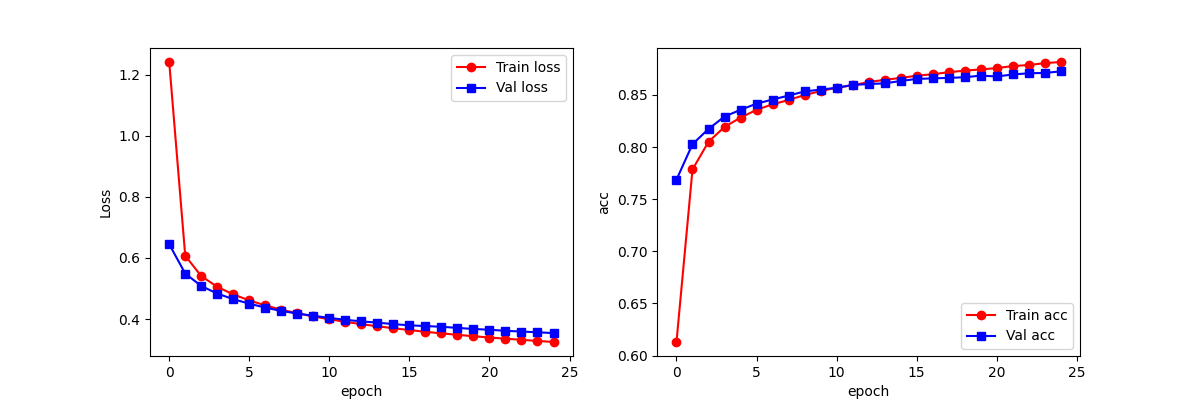
\includegraphics[width=1\linewidth]{CNN22.png}}
\heiti 图2.2\quad  训练结果(左图为loss曲线,右图为acc曲线)
\label{fig1}
\end{figure}

最终精确度(ACC)在测试集上为0.8711。

为了反应模型对不同类别的识别能力,生成了混淆矩阵,如图2.3所示。从图中可知模型对大多数类别可以精确的识别
唯一误差较大的类别是shirt,并且常把shirt识别为T-shirt,这是可以理解的,因为这两种类别的衣服确实有很高的相似度
如果需要更加精确的识别,可能需要增加更多的卷积层,识别更细微的特征。


\begin{figure}[htbp]
\centering
\vspace {-5mm}
\centerline{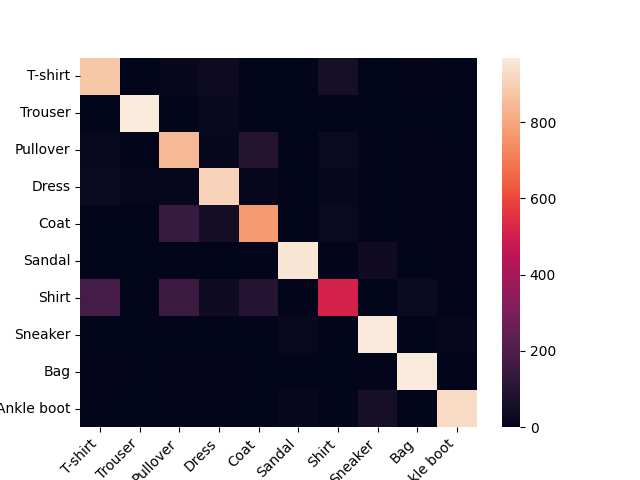
\includegraphics[width=0.7\linewidth]{CNN23.png}}
\heiti 图2.3\quad  混淆矩阵
\label{fig1}
\end{figure}


\subsubsection{不同网络结构的CNN对比}

在2.2.2节中我们已经构建了基础的CNN模型,但是在通常情况下的CNN模型中,会有更复杂的网络结构。
如更多的卷积层,更多的全连接层,为了比较不同网络结构下模型的性能,我们设置了一个对照组。
在训练模型2中我们设置了两个卷积层,设置了两个全连接层,在全连接层中设置了更多的神经元基础结构。
如图2.4所示,此次网络结构更为复杂,且分类器更深,其余参数与2.2.2中保持一致。

\begin{figure}[htbp]
\centering
\centerline{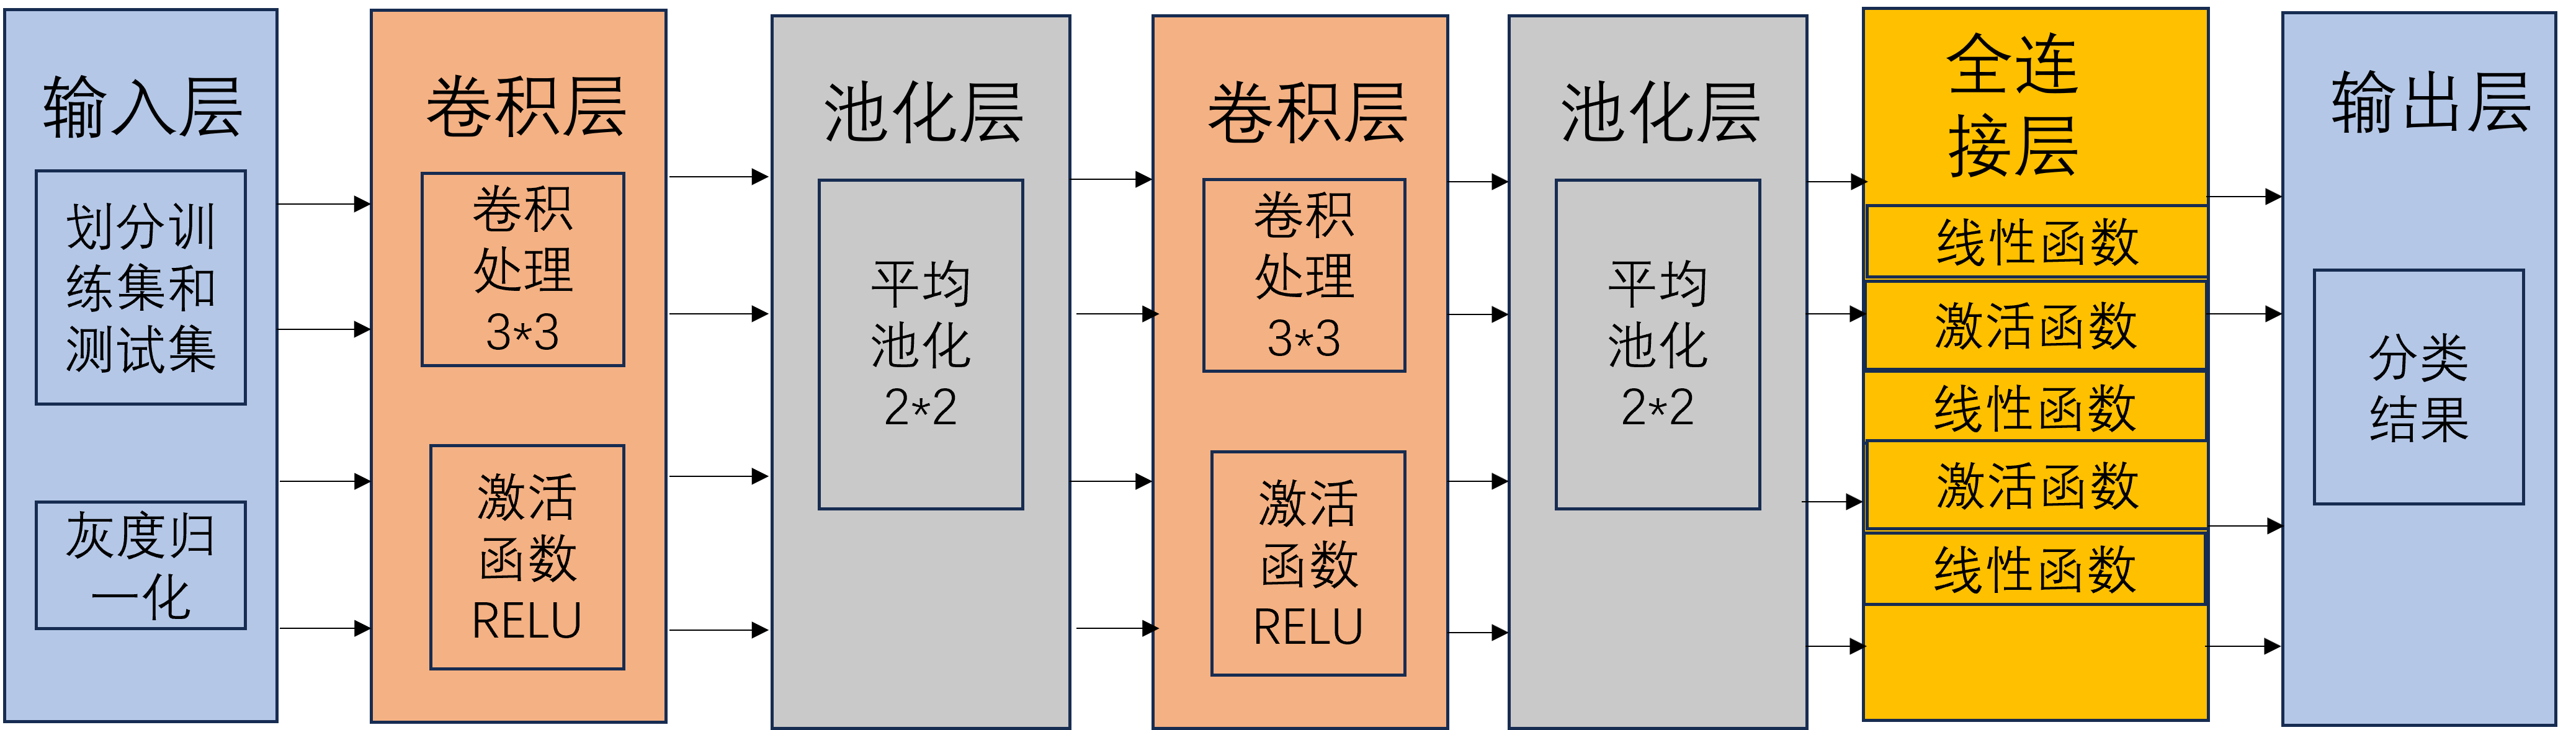
\includegraphics[width=1\linewidth]{CNN24.png}}
\heiti 图2.4\quad  不同的网络结构
\label{fig1}
\end{figure}

此次训练结果如图2.5所示,最终在测试集上的精确度为0.8619。
(简单模型下最终测试集的精确度为0.8711)


\begin{figure}[htbp]
\centering
\vspace {-8mm}
\centerline{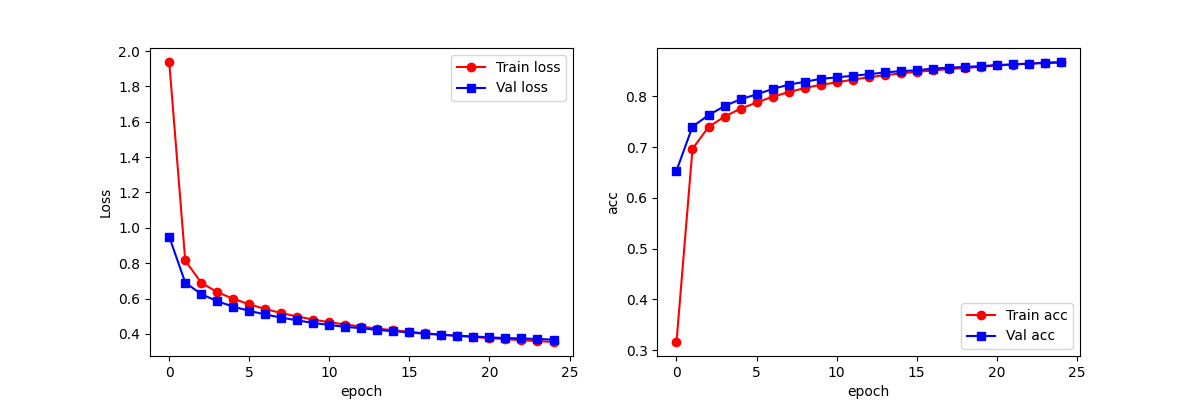
\includegraphics[width=1\linewidth]{CNN25.png}}
\heiti 图2.5\quad  训练结果(左图为loss曲线,右图为acc曲线)
\label{fig1}
\end{figure}
  
\vspace {-2mm}
从结果上来看,更复杂的结构并没有给网络性能带来明显的提升,
这可能是出于以下几点原因:

①FashionMNIST数据集中的数据本身是一个简单的数据集,简单的模型已经可以捕捉数据中的关键特征;

②更复杂的模型可能导致过拟合(这可能并没有发生,因为验证集和训练集并没有太多的误差);

③更复杂的模型通常需要更多的数据以及更长的训练时间,在此次训练中,由于训练数据不够多,可能导致模型训练不够充分;

④更复杂的模型参数更加敏感,这里可能没有调到合适的参数。例如可以修改滤波器核的大小,或者步长填充,池化方式等。


%%%%%%%%%%%%%%%%%%%%%%%%%%%%%%%%%%%%%%%5
%%%%%%%%%%%%%%%%%%%%%%%%%%%%%%%%%%%%%%%%%
\subsubsection{不同学习率的CNN对比}
在2.2.3节中我们分析了不同网络结构下CNN模型的对比,并且分析了复杂模型反而没有更好结果的原因。
通常学习率在机器学习中也会产生很大的影响,在上文的训练中学习率lr均为0.01,因此在本节中,分别改变在模型1(2.2.2中叙述的模型)和模型2(2.2.3中叙述的模型)的学习率,
比较结果并分析。

为了更明显看出不同参数间训练的结果,本次结果只展示在每个epoch中验证集上的结果,如图2.6所示。


\begin{figure}[htbp]
\centering
\vspace {-8mm}
\centerline{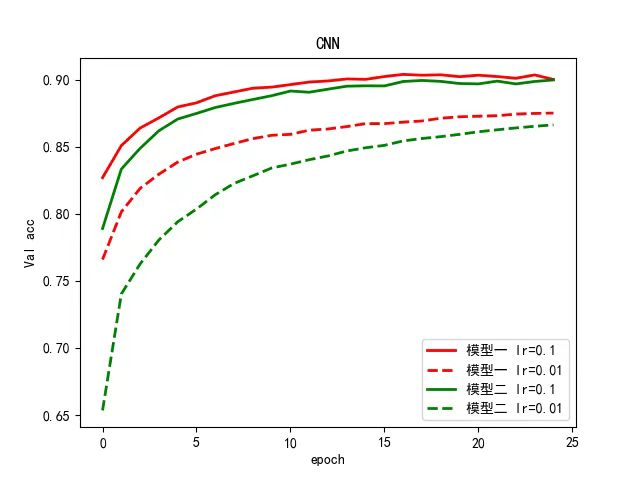
\includegraphics[width=0.7\linewidth]{CNN27.jpg}}
\heiti 图2.6\quad  不同训练模型以及学习率下的训练结果
\label{fig1}
\end{figure}

如图2.6所示,在相同的模型下,学习率lr越大,模型的收敛速度越快;
学习率lr低的时候会导致,acc提升的很慢。

但众所周知的是并不是学习率越大就一定越好,学习率越大,如图2.7所示说明了
在学习率过大的情况下对训练结果的影响,可能会导致参数一直在最低点附近振荡
无法到达最低点。

\begin{figure}[htbp]
\centering

\centerline{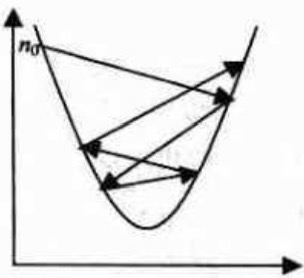
\includegraphics[width=0.5\linewidth]{CNN28.jpg}}
\heiti 图2.7\quad  不同训练模型以及学习率下的训练结果
\label{fig1}
\end{figure}

为了验证这一想法,我们在实验中再次增加模型一的学习率lr =0.5。得出的结果如图2.8所示:

\begin{figure}[htbp]
\centering

\centerline{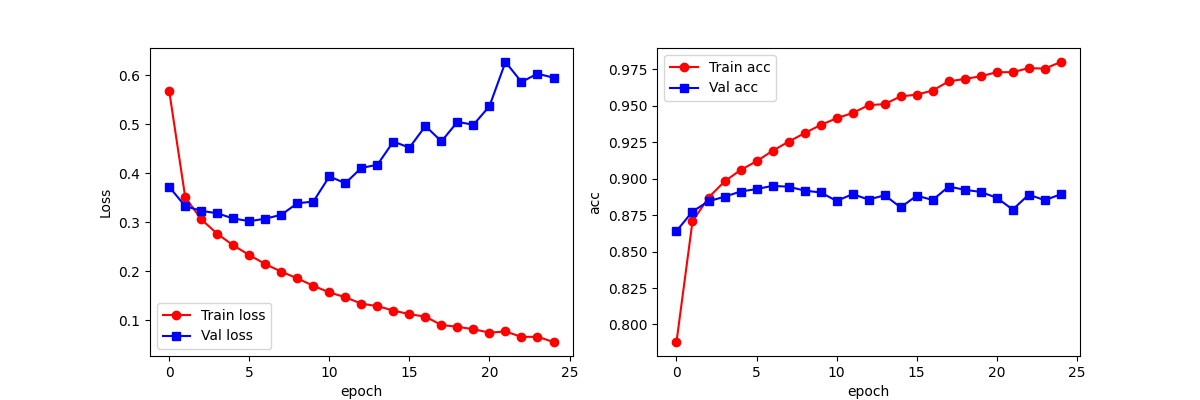
\includegraphics[width=1\linewidth]{CNN29.png}}
\heiti 图2.8\quad  模型一 lr=0.5时loss与acc曲线
\label{fig1}
\end{figure}

\vspace {-6mm}
正如上述的猜想,学习率lr过大时,acc与loss曲线来回振荡无法收敛,每一步的修改都可能错过最小值。
因此在机器学习中选择合适和学习率是一件至关重要的事情。

%%%%%%%%%%%%%%%%%%%%%%%%%%%%%%%%%%%%%%%5
%%%%%%%%%%%%%%%%%%%%%%%%%%%%%%%%%%%%%%%%%

\subsection{总结与优化}

在上文我们针对分类任务,使用了不同学习率以及不同网络结构的模型训练实现了这一任务,
并通过比较各个模型训练的精确率acc得出了很多结论。结构越复杂的网络不一定越好,
可能简单的数据集下简单的网络结构就可以实现很好的效果,结构复杂的网络反而可能导致参数过拟合。
从学习率的角度而言,学习率越高,模型的收敛速度越快,但到达一定界限的时候,较高的学习率会导致模型来回振荡
无法到达最低点或者说需要更多的时间才能够收敛;学习率越低,模型的收敛速度会变慢。

因此,CNN需要根据数据集选择合适的网络架构,同时在学习率的选择上也非常重要。
目前,出现了很多优化学习率的方式,我们采用自适应学习率(Adam,Adaptive Moment Estimation)的
方法对我们的模型进行优化。

Adam是一种常用的优化算法,
特别适用于训练神经网络和深度学习模型。
它是一种自适应学习率的优化算法,
可以根据不同参数的梯度信息来动态调整学习率,
以提高训练的效率和稳定性。
Adam算法的自适应性体现在:①动量(Momentum):Adam算法引入了动量项,类似于传统的动量优化算法。
②自适应学习率(Adaptive Learning Rate):Adam算法使用了每个参数的自适应学习率,这意味着不同参数可以具有不同的学习率。
优化后的结果如图2.9所示:

\begin{figure}[htbp]
\centering
\vspace {-6mm}
\centerline{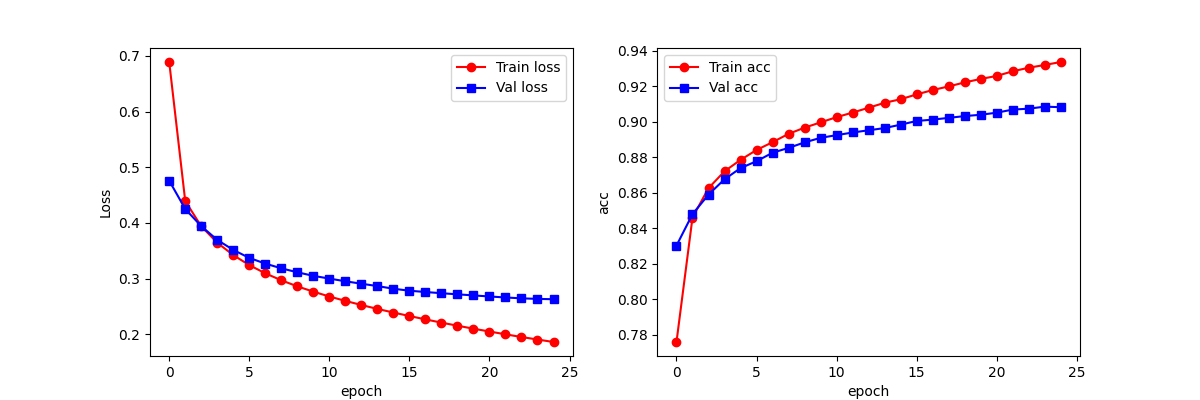
\includegraphics[width=1\linewidth]{CNN30.png}}
\heiti 图2.9\quad  模型一 引入Adam优化
\end{figure}
  
在引入Adam后,最终在测试集上的精度为0.8977,精度有了一定程度的提高。并且从图中我们也能看出
模型收敛的速度明显比之前要优。


%%%%%%%%%%%%%%%%%%%%%%%%%%%%%%%%5
%%%%%%%%%%%%%%%%%%%%%%%%%%%%%%%%%
\section{代码与展望}
本文第一章介绍了CNN网络以及其中各个层的基本作用;第二章针对此次的课程作业,详细对比了不同网络结构和不同学习率对网络训练的影响,
不仅如此在第二章中,我们发现了学习率过高引起的振荡问题,最后对学习率的问题作出了优化,引入了Adam自适应学习率,进一步提高了模型的
性能。
\subsection{代码}

我们的代码全部上传到github网址:https://github.com/mxwy/Machine-learning.git

\begin{figure}[htbp]
\centering

\centerline{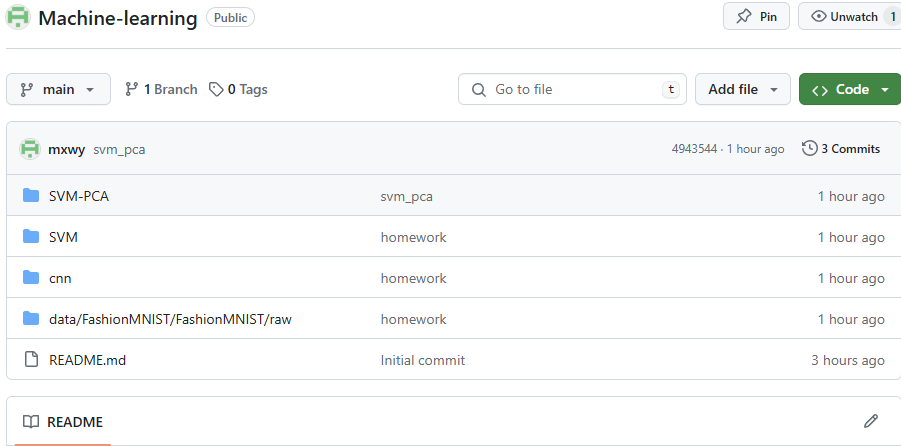
\includegraphics[width=0.8\linewidth]{github1.png}}
\heiti 图3.1\quad  Github库
\end{figure}

在README中我们对库中各个文件夹有着详细的描述以及运行方式,这里就不再赘述。

\begin{figure}[htbp]
\centering

\centerline{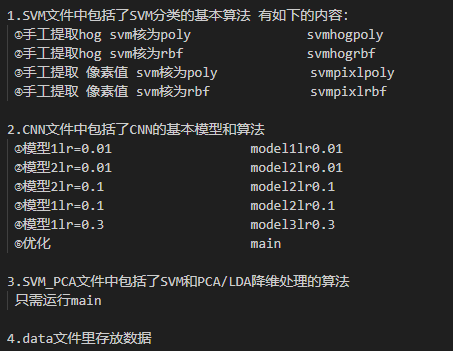
\includegraphics[width=0.5\linewidth]{github2.png}}
\heiti 图3.2\quad  README文件示例
\end{figure}


\subsection{展望}
尽管我们对此次分类任务,作出了较为完整的分析,但是还有很多不足亟待解决。

  1.通过混淆矩阵,我们知道,分类任务最易出现错误的地方在T-shirt和shirt之间,我们是否可以人工针对他们的区别,作出预处理。

  2.当图片发生旋转,对称等操作时,可能模型就不能很好的识别了,因此在数据预处理的时候可以加上旋转等操作,增加模型的容错性。

  3.此外本次分类任务主要针对此次课程作业且面向FashionMNIST数据集,在更大的数据集或更复杂的数据集下,需要更优的算法。

\subsection{分工占比}
本次课程作业闵昕贡献度占比为65$\%$(负责模型一三种不同的学习率以及自适应学习率优化部分的代码,负责编写技术报告),
王冠维占比为35$\%$(负责模型二两种不同的学习率)。




\vspace {10mm}
\zihao{5}{
\noindent \textsf{致\quad 谢}\quad \textit{ 感谢高飞老师在机器学习方面对我们提供的帮助,同时感谢前人对机器学习开创性的研究.}}

\vspace {10mm}
\centerline
{\zihao{5}\textsf{参~考~文~献}}
\zihao{5-} \addtolength{\itemsep}{-1em}
\vspace {1.5mm}
\bibliographystyle{gbt7714-numerical}
\bibliography{ref.bib}


\begin{thebibliography}{99}
  \zihao{5-} \addtolength{\itemsep}{-1em}
  \vspace {1.5mm}
  
  \bibitem{sunshineski2019}
  机器学习:混淆矩阵、准确率、错误率、灵敏度、特异度、精确度、召回率、F-Measure、ROC曲线、PR曲线,
  \textit{SunshineSki},
  2019年10月18日,
  \url{https://blog.csdn.net/SunshineSki/article/details/88078709}.
  
  \bibitem{adam2023}
  机器学习之Adam(Adaptive Moment Estimation)自适应学习率,
  \textit{奋进的大脑袋},
  2023年8月28日,
  \url{https://blog.csdn.net/qq_42244167/article/details/132476913}.

  \bibitem{adam2023}
  【机器学习300问】10、学习率设置过大或过小对训练有何影响?
  \textit{小oo呆},
  2024年03月14日,
  \url{https://blog.csdn.net/qq_39780701/article/details/135639802}.

  \bibitem{adam2023}
  基于CNN的FashionMNIST分类
  \textit{wangzaojun},
  2024年05月01日,
  \url{https://blog.csdn.net/m0_66504204/article/details/135076503}.

\end{thebibliography}



\end{document}


 